\documentclass[]{article}
\usepackage{lmodern}
\usepackage{amssymb,amsmath}
\usepackage{ifxetex,ifluatex}
\usepackage{fixltx2e} % provides \textsubscript
\ifnum 0\ifxetex 1\fi\ifluatex 1\fi=0 % if pdftex
  \usepackage[T1]{fontenc}
  \usepackage[utf8]{inputenc}
\else % if luatex or xelatex
  \ifxetex
    \usepackage{mathspec}
  \else
    \usepackage{fontspec}
  \fi
  \defaultfontfeatures{Ligatures=TeX,Scale=MatchLowercase}
\fi
% use upquote if available, for straight quotes in verbatim environments
\IfFileExists{upquote.sty}{\usepackage{upquote}}{}
% use microtype if available
\IfFileExists{microtype.sty}{%
\usepackage{microtype}
\UseMicrotypeSet[protrusion]{basicmath} % disable protrusion for tt fonts
}{}
\usepackage[margin=1in]{geometry}
\usepackage{hyperref}
\hypersetup{unicode=true,
            pdftitle={2018/08/23},
            pdfauthor={hane\_momiji},
            pdfborder={0 0 0},
            breaklinks=true}
\urlstyle{same}  % don't use monospace font for urls
\usepackage{color}
\usepackage{fancyvrb}
\newcommand{\VerbBar}{|}
\newcommand{\VERB}{\Verb[commandchars=\\\{\}]}
\DefineVerbatimEnvironment{Highlighting}{Verbatim}{commandchars=\\\{\}}
% Add ',fontsize=\small' for more characters per line
\usepackage{framed}
\definecolor{shadecolor}{RGB}{248,248,248}
\newenvironment{Shaded}{\begin{snugshade}}{\end{snugshade}}
\newcommand{\KeywordTok}[1]{\textcolor[rgb]{0.13,0.29,0.53}{\textbf{#1}}}
\newcommand{\DataTypeTok}[1]{\textcolor[rgb]{0.13,0.29,0.53}{#1}}
\newcommand{\DecValTok}[1]{\textcolor[rgb]{0.00,0.00,0.81}{#1}}
\newcommand{\BaseNTok}[1]{\textcolor[rgb]{0.00,0.00,0.81}{#1}}
\newcommand{\FloatTok}[1]{\textcolor[rgb]{0.00,0.00,0.81}{#1}}
\newcommand{\ConstantTok}[1]{\textcolor[rgb]{0.00,0.00,0.00}{#1}}
\newcommand{\CharTok}[1]{\textcolor[rgb]{0.31,0.60,0.02}{#1}}
\newcommand{\SpecialCharTok}[1]{\textcolor[rgb]{0.00,0.00,0.00}{#1}}
\newcommand{\StringTok}[1]{\textcolor[rgb]{0.31,0.60,0.02}{#1}}
\newcommand{\VerbatimStringTok}[1]{\textcolor[rgb]{0.31,0.60,0.02}{#1}}
\newcommand{\SpecialStringTok}[1]{\textcolor[rgb]{0.31,0.60,0.02}{#1}}
\newcommand{\ImportTok}[1]{#1}
\newcommand{\CommentTok}[1]{\textcolor[rgb]{0.56,0.35,0.01}{\textit{#1}}}
\newcommand{\DocumentationTok}[1]{\textcolor[rgb]{0.56,0.35,0.01}{\textbf{\textit{#1}}}}
\newcommand{\AnnotationTok}[1]{\textcolor[rgb]{0.56,0.35,0.01}{\textbf{\textit{#1}}}}
\newcommand{\CommentVarTok}[1]{\textcolor[rgb]{0.56,0.35,0.01}{\textbf{\textit{#1}}}}
\newcommand{\OtherTok}[1]{\textcolor[rgb]{0.56,0.35,0.01}{#1}}
\newcommand{\FunctionTok}[1]{\textcolor[rgb]{0.00,0.00,0.00}{#1}}
\newcommand{\VariableTok}[1]{\textcolor[rgb]{0.00,0.00,0.00}{#1}}
\newcommand{\ControlFlowTok}[1]{\textcolor[rgb]{0.13,0.29,0.53}{\textbf{#1}}}
\newcommand{\OperatorTok}[1]{\textcolor[rgb]{0.81,0.36,0.00}{\textbf{#1}}}
\newcommand{\BuiltInTok}[1]{#1}
\newcommand{\ExtensionTok}[1]{#1}
\newcommand{\PreprocessorTok}[1]{\textcolor[rgb]{0.56,0.35,0.01}{\textit{#1}}}
\newcommand{\AttributeTok}[1]{\textcolor[rgb]{0.77,0.63,0.00}{#1}}
\newcommand{\RegionMarkerTok}[1]{#1}
\newcommand{\InformationTok}[1]{\textcolor[rgb]{0.56,0.35,0.01}{\textbf{\textit{#1}}}}
\newcommand{\WarningTok}[1]{\textcolor[rgb]{0.56,0.35,0.01}{\textbf{\textit{#1}}}}
\newcommand{\AlertTok}[1]{\textcolor[rgb]{0.94,0.16,0.16}{#1}}
\newcommand{\ErrorTok}[1]{\textcolor[rgb]{0.64,0.00,0.00}{\textbf{#1}}}
\newcommand{\NormalTok}[1]{#1}
\usepackage{graphicx,grffile}
\makeatletter
\def\maxwidth{\ifdim\Gin@nat@width>\linewidth\linewidth\else\Gin@nat@width\fi}
\def\maxheight{\ifdim\Gin@nat@height>\textheight\textheight\else\Gin@nat@height\fi}
\makeatother
% Scale images if necessary, so that they will not overflow the page
% margins by default, and it is still possible to overwrite the defaults
% using explicit options in \includegraphics[width, height, ...]{}
\setkeys{Gin}{width=\maxwidth,height=\maxheight,keepaspectratio}
\IfFileExists{parskip.sty}{%
\usepackage{parskip}
}{% else
\setlength{\parindent}{0pt}
\setlength{\parskip}{6pt plus 2pt minus 1pt}
}
\setlength{\emergencystretch}{3em}  % prevent overfull lines
\providecommand{\tightlist}{%
  \setlength{\itemsep}{0pt}\setlength{\parskip}{0pt}}
\setcounter{secnumdepth}{0}
% Redefines (sub)paragraphs to behave more like sections
\ifx\paragraph\undefined\else
\let\oldparagraph\paragraph
\renewcommand{\paragraph}[1]{\oldparagraph{#1}\mbox{}}
\fi
\ifx\subparagraph\undefined\else
\let\oldsubparagraph\subparagraph
\renewcommand{\subparagraph}[1]{\oldsubparagraph{#1}\mbox{}}
\fi

%%% Use protect on footnotes to avoid problems with footnotes in titles
\let\rmarkdownfootnote\footnote%
\def\footnote{\protect\rmarkdownfootnote}

%%% Change title format to be more compact
\usepackage{titling}

% Create subtitle command for use in maketitle
\newcommand{\subtitle}[1]{
  \posttitle{
    \begin{center}\large#1\end{center}
    }
}

\setlength{\droptitle}{-2em}
  \title{2018/08/23}
  \pretitle{\vspace{\droptitle}\centering\huge}
  \posttitle{\par}
  \author{hane\_momiji}
  \preauthor{\centering\large\emph}
  \postauthor{\par}
  \predate{\centering\large\emph}
  \postdate{\par}
  \date{2018/8/23}


\begin{document}
\maketitle

{
\setcounter{tocdepth}{2}
\tableofcontents
}
\section{今日やったことまとめ}

今日は基本的に、dplyr, tidyrによるtidy
dataの作り方の続きからスタートし、ggplot2, RMarkdownの導入を行った。
本を終えたので、昨日勉強したスクレイピングで取得した為替データを整形し、ggplot2で出力するところまで行った。
一先ず、スクレイピングでつまづいた箇所をまとめておく。

本日使ったパッケージはこちら

\href{https://kabutan.jp/stock/kabuka?code=0950}{カブタン}からデータを取得してくるのは本とほぼ同様で、
chromeの検証機能を使ってXPathを取得し、貼り付けた。次回以降の利用を考え関数としてまとめた。

\paragraph{データ取得の関数}

\begin{Shaded}
\begin{Highlighting}[]
\CommentTok{# 連番のURL取得}
\NormalTok{renban_url <-}\StringTok{ }\ControlFlowTok{function}\NormalTok{(base_url, n)\{}
\NormalTok{  urls <-}\StringTok{ }\OtherTok{NULL}
  \ControlFlowTok{for}\NormalTok{ (i }\ControlFlowTok{in} \DecValTok{1}\OperatorTok{:}\NormalTok{n)\{}
\NormalTok{    pgnum <-}\StringTok{ }\KeywordTok{as.character}\NormalTok{(i)}
\NormalTok{    urls[i] <-}\StringTok{ }\KeywordTok{paste0}\NormalTok{(base_url, pgnum)}
\NormalTok{  \}}
  \KeywordTok{return}\NormalTok{(urls)}
\NormalTok{\}}

\CommentTok{# 連番URLを入れると、表をダウンロードする}
\NormalTok{renban_dl <-}\StringTok{ }\ControlFlowTok{function}\NormalTok{(base_url, n, }\DataTypeTok{XPath =} \StringTok{'//*[@id="stock_kabuka_table"]/table[2]'}\NormalTok{)\{}
\NormalTok{  urls <-}\StringTok{ }\KeywordTok{renban_url}\NormalTok{(base_url, n)}
\NormalTok{  kawases <-}\StringTok{ }\KeywordTok{list}\NormalTok{()}
  \ControlFlowTok{for}\NormalTok{ (i }\ControlFlowTok{in} \DecValTok{1}\OperatorTok{:}\NormalTok{n)\{}
\NormalTok{    memory <-}\StringTok{ }\KeywordTok{read_html}\NormalTok{(urls[i]) }\OperatorTok\StringTok{ }
\StringTok{      }\KeywordTok{html_nodes}\NormalTok{(}\DataTypeTok{xpath =}\NormalTok{ XPath) }\OperatorTok\StringTok{ }
\StringTok{      }\KeywordTok{html_table}\NormalTok{() }\OperatorTok\StringTok{ }
\StringTok{      }\KeywordTok{as.data.frame}\NormalTok{() }\OperatorTok\StringTok{ }
\StringTok{      }\NormalTok{dplyr}\OperatorTok{::}\KeywordTok{mutate_at}\NormalTok{(}\StringTok{"前日比"}\NormalTok{, as.numeric) }\OperatorTok\StringTok{ }
\StringTok{      }\NormalTok{dplyr}\OperatorTok{::}\KeywordTok{mutate_at}\NormalTok{(}\StringTok{"前日比."}\NormalTok{, as.numeric) }
\NormalTok{    memory[,}\StringTok{"日付"}\NormalTok{] <-}\StringTok{ }\KeywordTok{parse_date}\NormalTok{(memory[, }\StringTok{"日付"}\NormalTok{], }\StringTok{"%x"}\NormalTok{)}
\NormalTok{    kawases[[i]] <-}\StringTok{ }\NormalTok{memory}
    \KeywordTok{Sys.sleep}\NormalTok{(}\FloatTok{0.5}\NormalTok{)}
\NormalTok{  \}}
  \KeywordTok{return}\NormalTok{(kawases)}
\NormalTok{\}}
\end{Highlighting}
\end{Shaded}

上の関数で、\texttt{renban\_dl}で本と大きく変えている点は、\\
- ``前日比''の型が数値型になっている点\\
- ``日付''を文字列型ではなく、POSIXctに変換してから取得している点\\
である。最後に、これについてまとめておく。

これで、スクレイピングの処理は書けたので動かしてみると以下のようになる。

\begin{Shaded}
\begin{Highlighting}[]
\NormalTok{kawases_url <-}\StringTok{ "https://kabutan.jp/stock/kabuka?code=0950&ashi=day&page="}
\NormalTok{dat <-}\StringTok{ }\KeywordTok{renban_dl}\NormalTok{(kawases_url, }\DecValTok{10}\NormalTok{)}
\NormalTok{data <-}\StringTok{ }\KeywordTok{list}\NormalTok{()}
\NormalTok{data <-}\StringTok{ }\NormalTok{dplyr}\OperatorTok{::}\KeywordTok{bind_rows}\NormalTok{(dat)}
\KeywordTok{write_csv}\NormalTok{(data, }\StringTok{"kawase/kawase.csv"}\NormalTok{)}
\NormalTok{font <-}\StringTok{ "HiraKakuPro-W3"}
\KeywordTok{ggplot}\NormalTok{(}\DataTypeTok{data =}\NormalTok{ data, }\DataTypeTok{family =}\NormalTok{ font) }\OperatorTok{+}
\StringTok{  }\KeywordTok{geom_line}\NormalTok{(}\DataTypeTok{mapping =} \KeywordTok{aes}\NormalTok{(}\DataTypeTok{x =}\NormalTok{ 日付, }\DataTypeTok{y =}\NormalTok{ 終値)) }\OperatorTok{+}
\StringTok{  }\KeywordTok{theme}\NormalTok{(}\DataTypeTok{text =} \KeywordTok{element_text}\NormalTok{(}\DataTypeTok{family =}\NormalTok{ font)) }\OperatorTok{+}
\StringTok{  }\KeywordTok{scale_fill_brewer}\NormalTok{(}\DataTypeTok{palette =} \StringTok{"Paired"}\NormalTok{)}
\end{Highlighting}
\end{Shaded}

しかし、これではtidy
dataになっていないので、プロットする時もY軸に終値・高値・安値・始値を
取らなくてはならない。これを、4種類の値段ごとに色分けして一つのプロットの中に描画する事が
一応今日の目標であった。\\
tidyな形に直してみると、このようになって、4つの値段の名前をkeyにしてlong
formにすることができた。

\begin{Shaded}
\begin{Highlighting}[]
\NormalTok{d <-}\StringTok{ }\NormalTok{data }\OperatorTok\StringTok{ }
\StringTok{  }\NormalTok{dplyr}\OperatorTok{::}\KeywordTok{select}\NormalTok{(日付}\OperatorTok{:}\NormalTok{終値)}
\NormalTok{data_tidy <-}\StringTok{ }\KeywordTok{gather}\NormalTok{(d, }\DataTypeTok{key =} \StringTok{"name"}\NormalTok{, }\DataTypeTok{value =} \StringTok{"exchange_rate"}\NormalTok{,}
\NormalTok{                    始値,高値,安値,終値)}
\KeywordTok{ggplot}\NormalTok{(}\DataTypeTok{data =}\NormalTok{ data_tidy, }\DataTypeTok{family =}\NormalTok{ font) }\OperatorTok{+}
\StringTok{  }\KeywordTok{geom_line}\NormalTok{(}\DataTypeTok{mapping =} \KeywordTok{aes}\NormalTok{(}\DataTypeTok{x =}\NormalTok{ 日付, }\DataTypeTok{y =}\NormalTok{ exchange_rate, }\DataTypeTok{colour =}\NormalTok{ name)) }\OperatorTok{+}
\StringTok{  }\KeywordTok{theme}\NormalTok{(}\DataTypeTok{text =} \KeywordTok{element_text}\NormalTok{(}\DataTypeTok{family =}\NormalTok{ font)) }\OperatorTok{+}
\StringTok{  }\KeywordTok{scale_colour_brewer}\NormalTok{(}\DataTypeTok{palette =} \StringTok{"Paired"}\NormalTok{)}
\end{Highlighting}
\end{Shaded}

plotした結果を貼ると 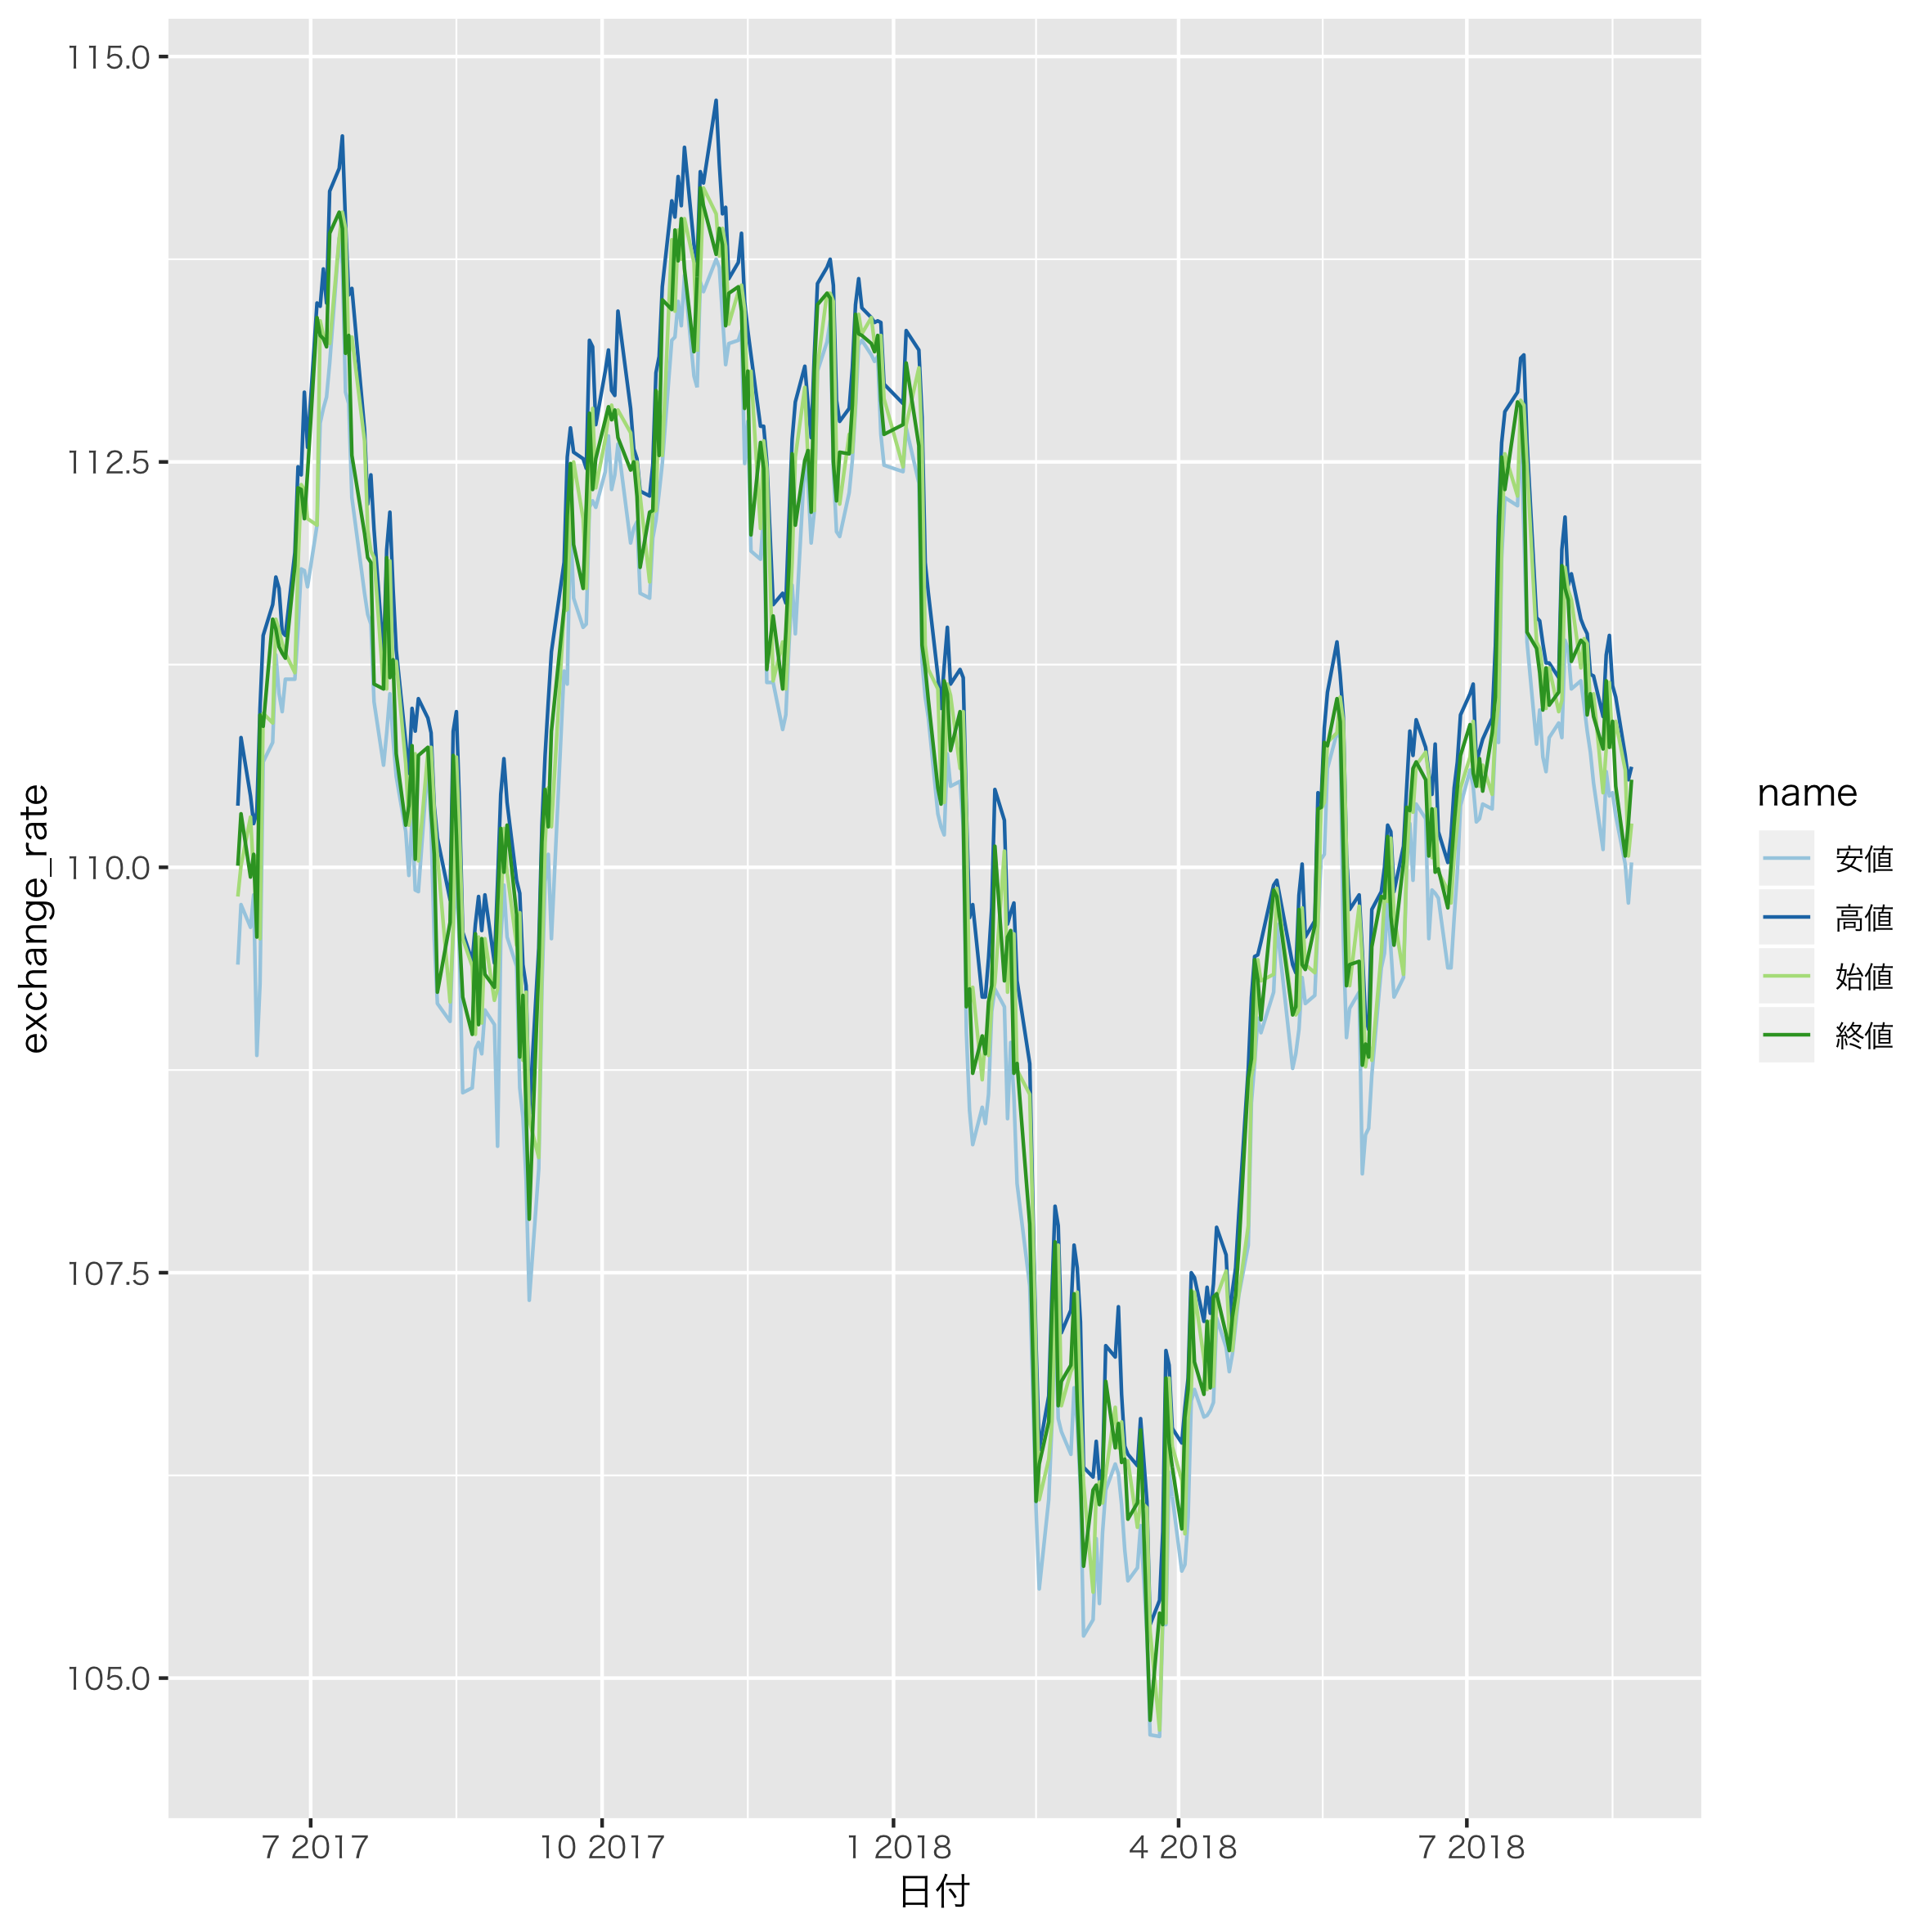
\includegraphics{yen-dollar.png}

\subsection{型を揃えてtibbleを連結する}\label{tibble}

最後に、今回少し苦労した変換の方法についてまとめておく。\\
まず、``前日比'',``前日比.''のカラムには基本的に数値で入っているが、10ページ目には文字列で入っていた。
それは、一番最初の日付には前日のデータが存在しないためにハイフンが含まれていたからだと思われる。
その為、これは無視して\texttt{as.numeric()}に代入すれば、最終行以外はすんなり数値型にしてくれて、最終行は
NAで処理してくれる。

\subsection{文字列型で書かれた日付をPOSIXctに変換する方法}\label{posixct}

そして、1番重要な文字列型の日付を直す方法であるが、今回使った\emph{parse\_date(x,
format = ``'')}は\textbf{readr}パッケージに入っている。\\
xにベクトルを入れて、formatで文字列がどういう規則で日付を表しているかを指定している。具体的には\\
- Year: ``\%Y'' (4 digits). ``\%y'' (2 digits); 00-69 -\textgreater{}
2000-2069, 70-99 -\textgreater{} 1970-1999.

\begin{itemize}
\item
  Month: ``\%m'' (2 digits), ``\%b'' (abbreviated name in current
  locale), ``\%B'' (full name in current locale).
\item
  Day: ``\%d'' (2 digits), ``\%e'' (optional leading space)
\item
  Hour: ``\%H'' or ``\%I'', use I (and not H) with AM/PM.
\item
  Minutes: ``\%M''
\item
  Seconds: ``\%S'' (integer seconds), ``\%OS'' (partial seconds)
\item
  Time zone: ``\%Z'' (as name, e.g. ``America/Chicago''), ``\%z'' (as
  offset from UTC, e.g. ``+0800'')
\item
  AM/PM indicator: ``\%p''.
\item
  Shortcuts: ``\%D'' = ``\%m/\%d/\%y'', ``\%F'' = ``\%Y-\%m-\%d'',
  ``\%R'' = ``\%H:\%M'', ``\%T'' = ``\%H:\%M:\%S'', ``\%x'' =
  ``\%y/\%m/\%d''.
\end{itemize}

というような形で、指定している。今回は18/08/23というような形式だったので\texttt{"\%y/\%m/\%d"}または\texttt{"\%x"}というformatになった。
その他の関数については\href{https://heavywatal.github.io/rstats/readr.html}{このサイト}が参考になる。


\end{document}
